\chapter{Tasks}
In this chapter we are going to provide, thanks to a Gantt chart, a high-level project schedule, defining all main tasks necessary for developing the project. Even if in reality we worked only on RASD, DD, ITPD and PPD, because of the didactic purpose of the project, we decided to provide also the time necessary for developing, testing and finally deploying the system, also using results obtained with COCOMO II analysis.

\begin{figure}[H]
	\centering
	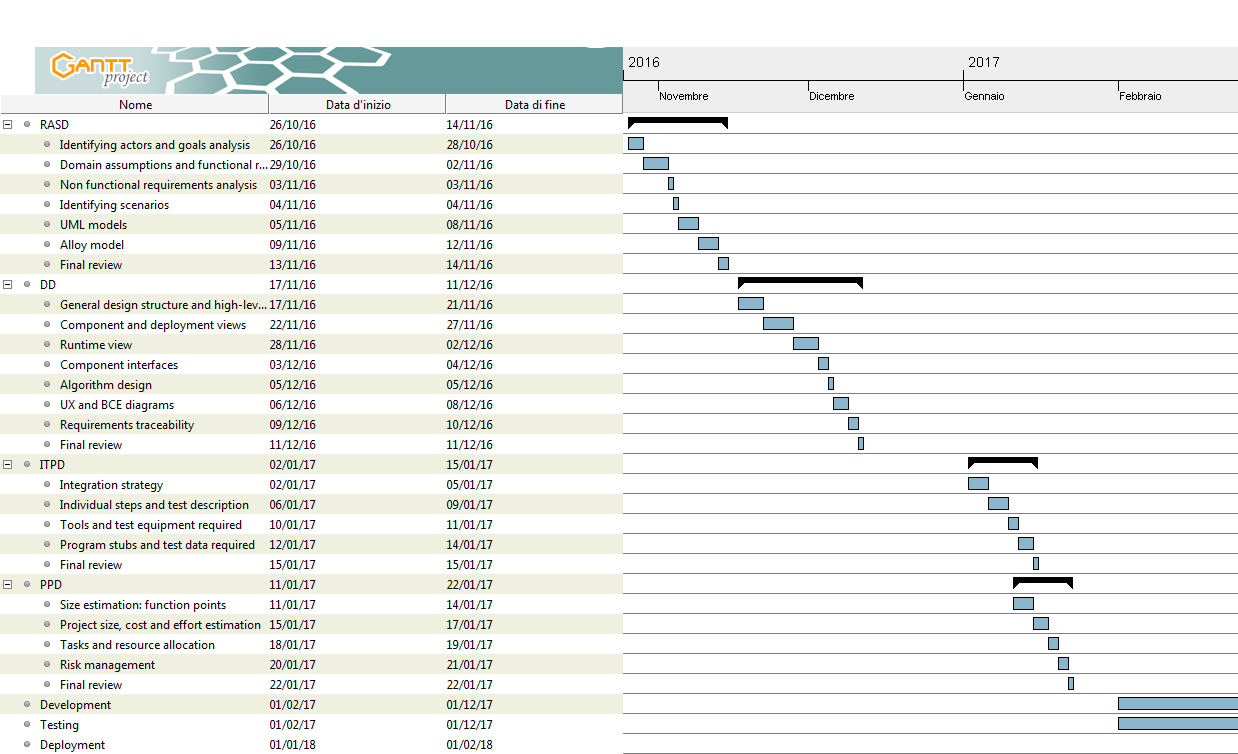
\includegraphics[width=1\textwidth]{Tasks1}
	\caption[Tasks-1]{The picture above shows the first section of Gantt chart representing main tasks of the project.}
	\label{fig:Tasks-1}
\end{figure}

\begin{figure}[H]
	\centering
	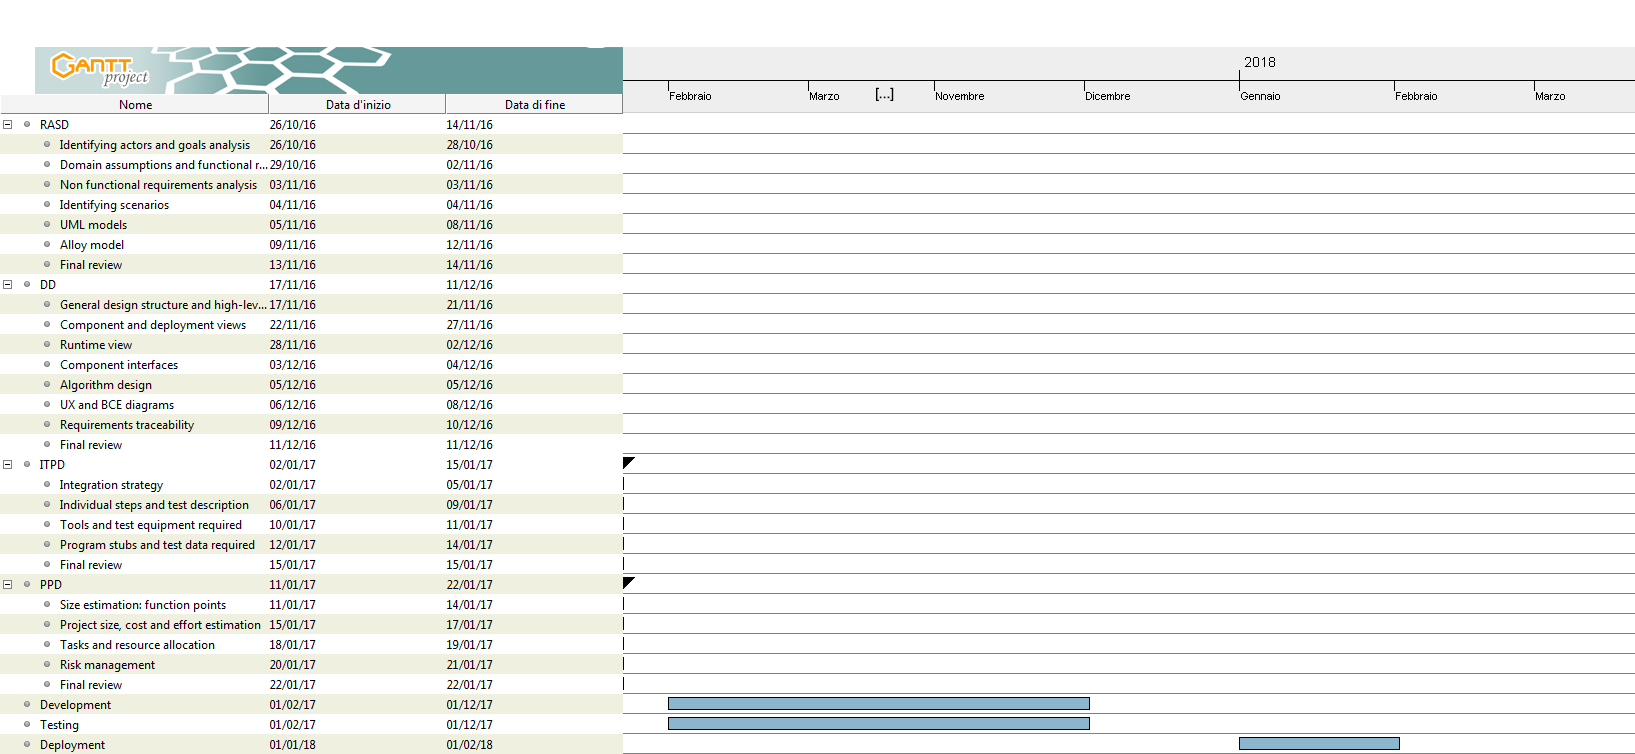
\includegraphics[width=1\textwidth]{Tasks2}
	\caption[Tasks-1]{The picture above shows the second section of Gantt chart representing main tasks of the project.}
	\label{fig:Tasks-2}
\end{figure}